
% This thesis template is based on the report class of
% latex. Yout do not need to change this.
\documentclass[12pt, a4paper]{report}

% This includes all variables that are used in this work
% Use this document to specify your name, your reviewers
% and other values that you would like to maintain
% in one place.
\newcommand\myname{Paul Leitner, BA}
\newcommand\mypkz{1910837299}

\newcommand\myfirstreviewer{Prof. (FH) Dr. Johannes Lüthi}
% Leave second review empty for bachelor's thesis
\newcommand\mysecondreviewer{Prof. (FH) PD Dr. Mario Döller}

\newcommand\mytitle{A history of Artificial Neural Networks}

% The value below is the date that you finished your work. This
% date appears on you work's cover page and in the "Eidesstattliche
% Erklärung".
\newcommand\mydate{31. October 2021}

% For a master's thesis use MA as type, BA for a bachelor's thesis
\newcommand\type{MA}

% Set the name of your study program. 
% DSIA for Data Science & Intelligent Analytics
% WEB for Web Business & Technology
% WCIS for Web Communications and Information Systems
% SPS for Smart Products and Solutions
\newcommand\program{DSIA}

% Define the language in which you write this thesis
% Use DE for German, EN for English
\newcommand\lang{EN}


% This includes all packages and presets. You do not need
% to change this file unless you want to add new packages
% or change the presets of one of the used packages.
\usepackage{pxfonts}
\usepackage[T1]{fontenc}
\usepackage{graphicx}
\usepackage[utf8]{inputenc}
\usepackage{blindtext}  % Used for dummy text segments
\usepackage{natbib}
\usepackage{hyperref}
\usepackage{booktabs}
\usepackage{xcolor}
\usepackage{ifthen}
\usepackage{xspace}
\usepackage{acronym}

\ifthenelse{\equal{\lang}{DE}}{
    \usepackage[ngerman]{babel} 
}{
    \usepackage[english]{babel} 
}

\usepackage{listings}
\lstset{numberbychapter=false}
\iflanguage{english}{
  \renewcommand{\lstlistlistingname}{List of Listings}
  \newcommand{\lstacronymname}{List of Acronyms}
  }{
  \renewcommand{\lstlistlistingname}{Listingsverzeichnis}
  \newcommand{\lstacronymname}{Abkürzungsverzeichnis}
}

\usepackage{fancyhdr}  % Head and footer styling
\fancyhead[RO]{\thepage}
\fancyhead[LO]{\nouppercase\leftmark}
\renewcommand\headrulewidth{0.5pt}
\renewcommand\footrulewidth{0pt}

\usepackage[a4paper, left=3.5cm, right=3cm, top=3.5cm, bottom=3cm]{geometry}
\setlength{\headheight}{15pt}

\usepackage[title, titletoc, header]{appendix}
\renewcommand{\appendixname}{Appendix}

\usepackage{titlesec}
\titleformat{\chapter}{\bf \LARGE}{\thechapter.}{16pt}{\LARGE}

\usepackage{chngcntr}
\counterwithout{figure}{chapter}
\counterwithout{table}{chapter}

% Check for work type
\ifthenelse{\equal{\type}{MA}}{
    \newcommand\academictitle{Master of Science in Engineering (M.Sc.)}
    \newcommand\worktype{Masterarbeit\xspace}
}{
    \newcommand\academictitle{Bachelor of Science in Engineering (B.Sc.)}
    \newcommand\worktype{Bachelorarbeit\xspace}
}

% Check for study program 
\ifthenelse{\equal{\program}{DSIA}}{
    \newcommand\studyprogram{Data Science \& Intelligent Analytics}
}{
    \ifthenelse{\equal{\program}{WEB}}{
        \newcommand\studyprogram{Web Business \& Technology}
    }{
        \ifthenelse{\equal{\program}{WCIS}}{
            \newcommand\studyprogram{Web Communication \& Information Systems}
        }{
            \newcommand\studyprogram{Smart Products \& Solutions}
        }
    }
}


\pagestyle{headings}
\setlength{\parindent}{0em}
\setlength{\parskip}{1em}
\renewcommand{\baselinestretch}{1.5}

\newcommand\frontmatter{
    \pagestyle{fancy}
    \fancyfoot{}
    \pagenumbering{Roman}
}

\newcommand\mainmatter{
    \pagenumbering{arabic}
}

\newcommand\backmatter{
    \pagenumbering{arabic}
    \renewcommand{\thepage}{A\arabic{page}}
}        

\lstset{
    numberstyle=\tiny,
    numbers=left,
    showstringspaces=false,
    breaklines=true,
    commentstyle=\itshape\color{darkgray},
    basicstyle=\ttfamily,
    stringstyle=\color{orange},
    keywordstyle=\bf\color{green!40!black},
    identifierstyle=\color{blue}
}

% add support for JavaScript as per https://github.com/ghammock/LaTeX_Listings_JavaScript_ES6
% Kudos to Guni

\lstdefinelanguage[ECMAScript2015]{JavaScript}[]{JavaScript}{
  morekeywords=[1]{await, async, case, catch, class, const, default, do,
    enum, export, extends, finally, from, implements, import, instanceof,
    let, static, super, switch, throw, try},
  morestring=[b]` % Interpolation strings.
}

\lstdefinelanguage{JavaScript}{
  morekeywords=[1]{async, await, break, continue, delete, else, for, function, if, in,
    new, return, this, typeof, var, void, while, with},
  % Literals, primitive types, and reference types.
  morekeywords=[2]{false, null, true, boolean, number, undefined,
    Array, Boolean, Date, Math, Number, String, Object},
  % Built-ins.
  morekeywords=[3]{eval, parseInt, parseFloat, escape, unescape, forEach, map, filter, reduce},
  sensitive,
  morecomment=[s]{/*}{*/},
  morecomment=[l]//,
  morecomment=[s]{/**}{*/}, % JavaDoc style comments
  morestring=[b]',
  morestring=[b]"
}[keywords, comments, strings]

\lstalias[]{ES6}[ECMAScript2015]{JavaScript}

% Requires package: color.
\definecolor{mediumgray}{rgb}{0.3, 0.4, 0.4}
\definecolor{mediumblue}{rgb}{0.0, 0.0, 0.8}
\definecolor{forestgreen}{rgb}{0.13, 0.55, 0.13}
\definecolor{darkviolet}{rgb}{0.58, 0.0, 0.83}
\definecolor{royalblue}{rgb}{0.25, 0.41, 0.88}
\definecolor{crimson}{rgb}{0.86, 0.8, 0.24}

\lstdefinestyle{JSES6Base}{
  backgroundcolor=\color{white},
  basicstyle=\ttfamily,
  breakatwhitespace=false,
  breaklines=false,
  captionpos=b,
  columns=fullflexible,
  commentstyle=\color{mediumgray}\upshape,
  emph={},
  emphstyle=\color{crimson},
  extendedchars=true,  % requires inputenc
  fontadjust=true,
  frame=single,
  identifierstyle=\color{black},
  keepspaces=true,
  keywordstyle=\color{mediumblue},
  keywordstyle={[2]\color{darkviolet}},
  keywordstyle={[3]\color{royalblue}},
  numbers=left,
  numbersep=5pt,
  numberstyle=\tiny\color{black},
  rulecolor=\color{black},
  showlines=true,
  showspaces=false,
  showstringspaces=false,
  showtabs=false,
  stringstyle=\color{forestgreen},
  tabsize=2,
  title=\lstname,
  upquote=true  % requires textcomp
}

\lstdefinestyle{JavaScript}{
  language=JavaScript,
  style=JSES6Base
}
\lstdefinestyle{ES6}{
  language=ES6,
  style=JSES6Base
}

\hypersetup{
  pdftitle    = \mytitle,
  pdfsubject  = \worktype,
  pdfauthor   = \myname,
  pdfcreator  = {pdflatex using template provided by University of Applied Sciences FH Kufstein Tirol},
  bookmarksnumbered = true,
  colorlinks = true,
  linkcolor = blue,
  citecolor = green,
  urlcolor = orange
}


% This includes custom latex commands. You can use this
% file to create your own command sequences.
\newcommand{\fh}{\textsc{FH Kufstein Tirol}}

\newcommand{\fig}[4]{
    \begin{figure}[ht]
        \centering
        \includegraphics[width=#4\textwidth]{#1}
        \caption{#2}
        \label{#3}
    \end{figure}
}



\begin{document}

    \frontmatter

    % This places the front matter. You do not need to 
    % change this file. All thesis-specific values are 
    % imported from "variables.tex".
    \begin{titlepage}
 
    \vfill
    \begin{center}
      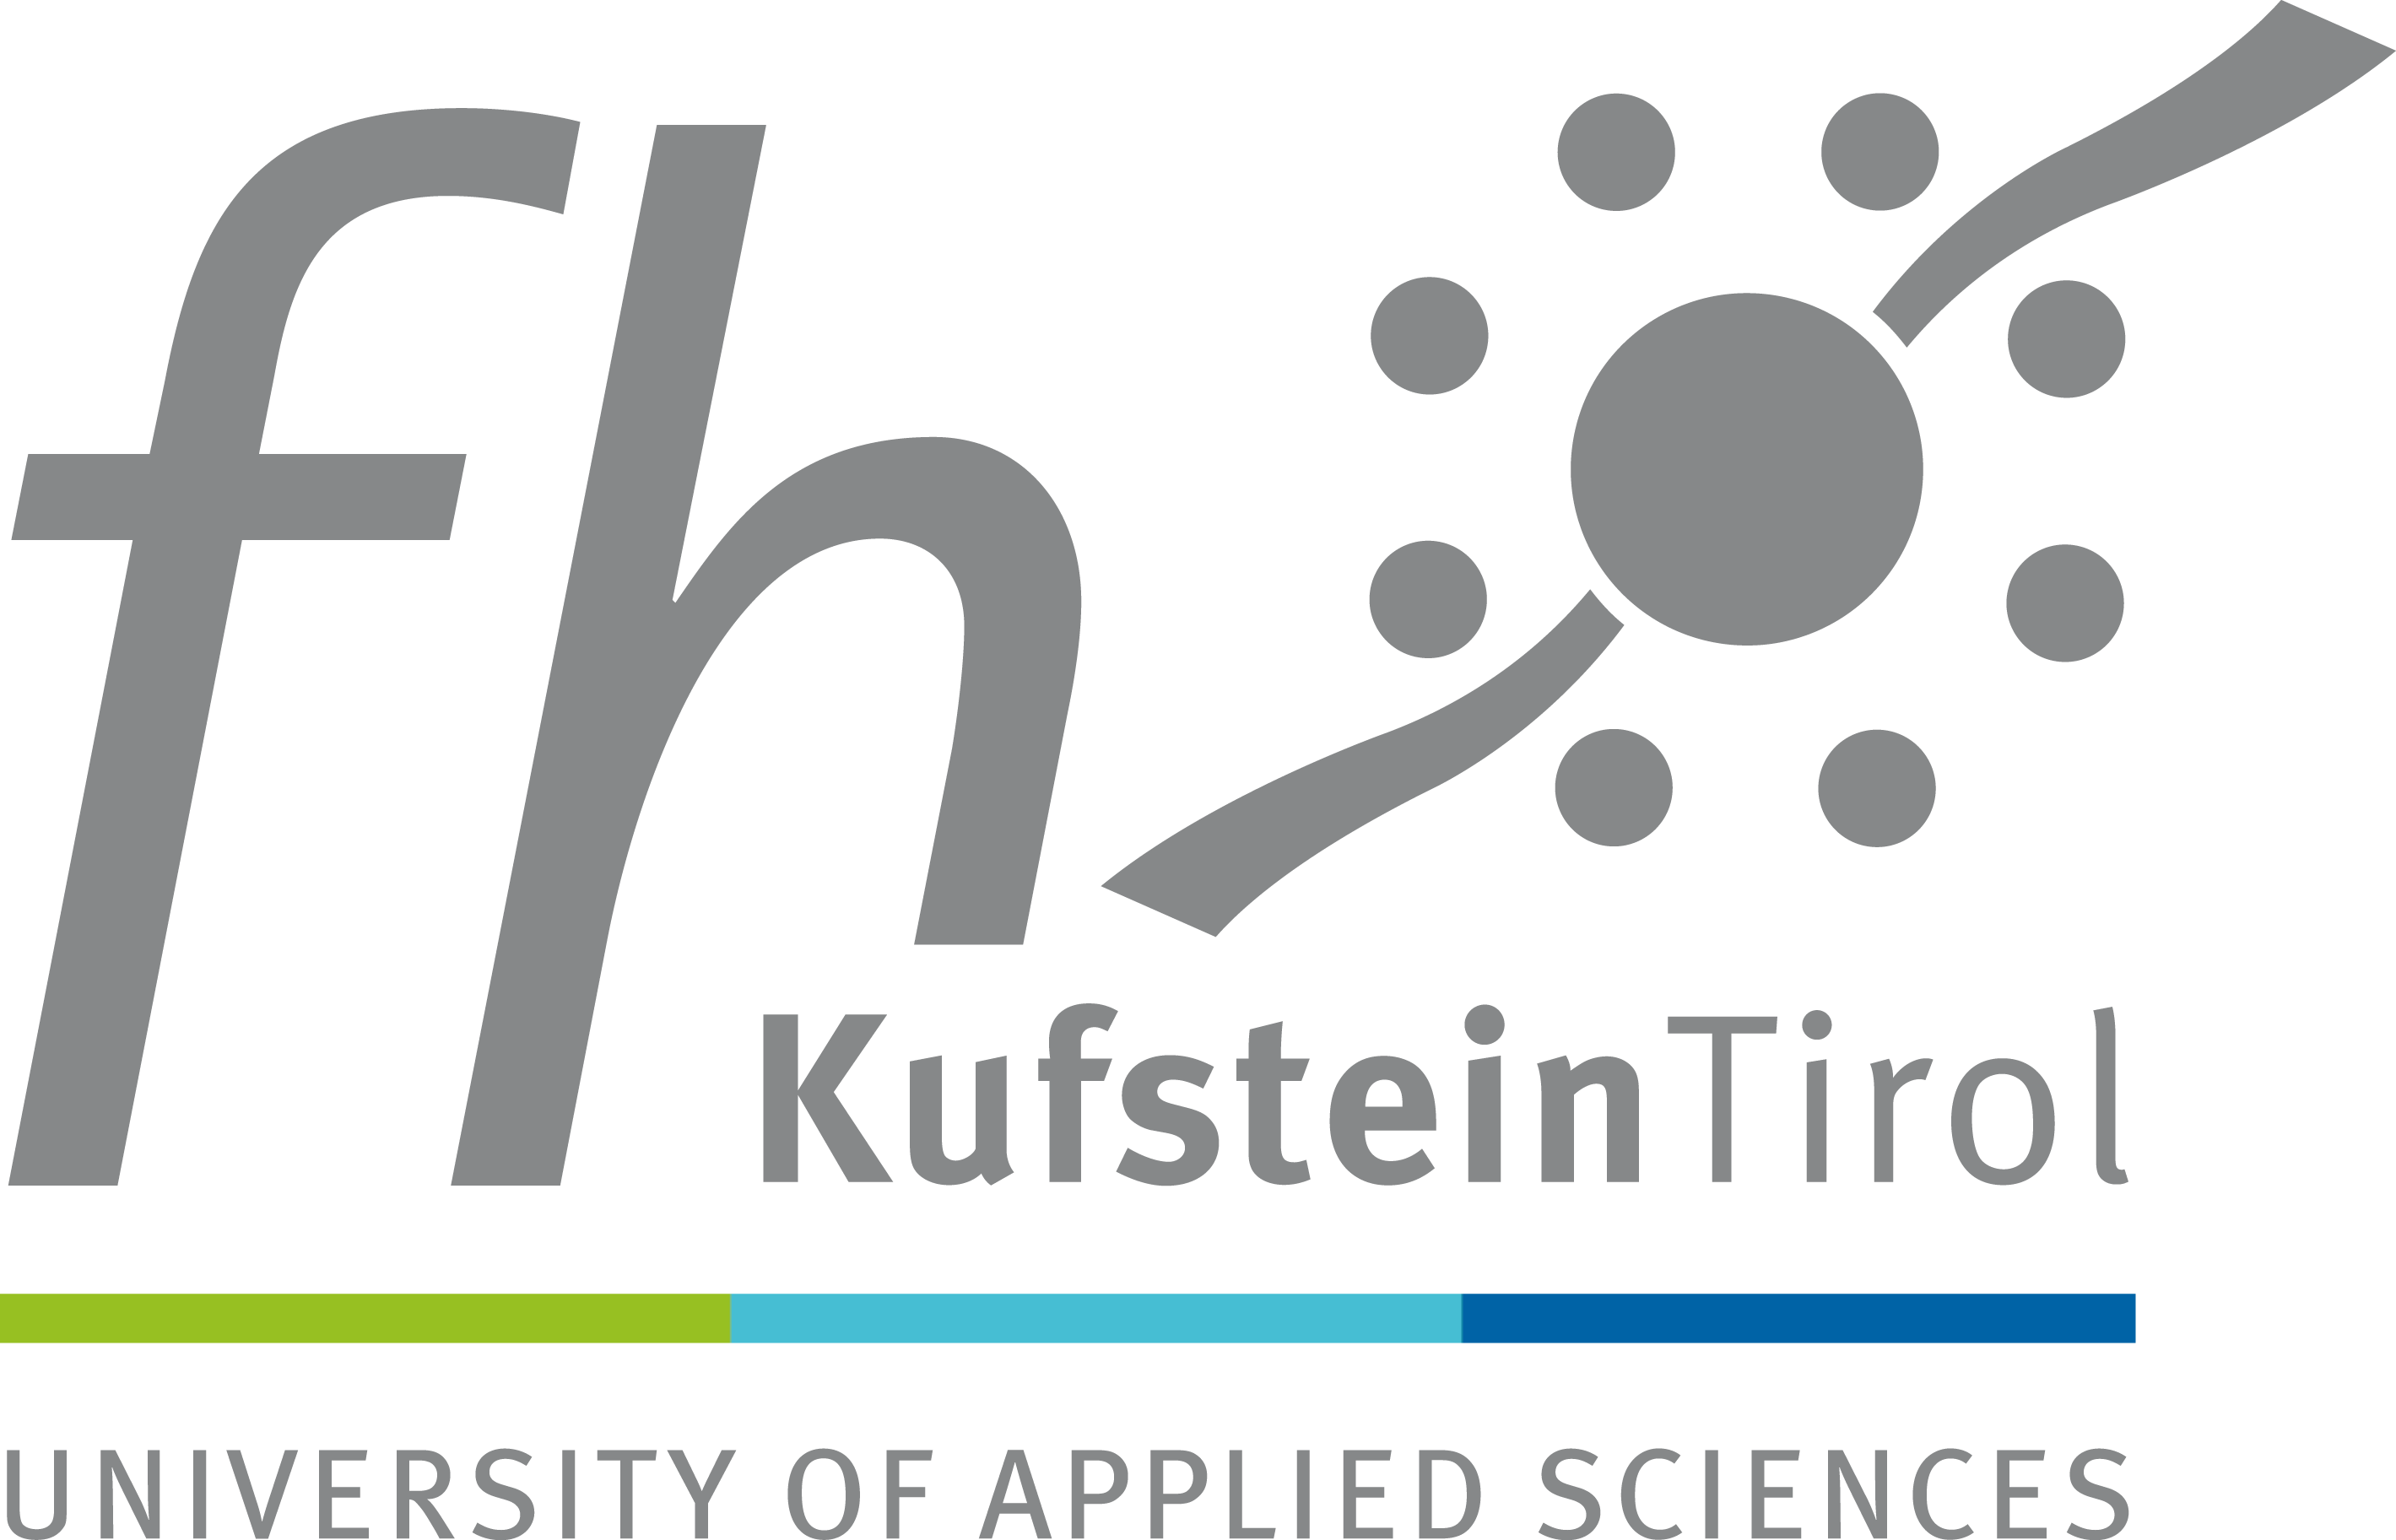
\includegraphics[width=4.5cm]{img/kufstein_logo.png} \\ 
    \end{center}
    \vfill
  
    \begin{center}
      \Large \textbf{\mytitle}
    \end{center} 
    \vfill
  
%    \begin{center}
      %\condMASTER{\Large Masterarbeit}{\Large Bachelorarbeit}
%      \worktype
%    \end{center}
%    \vfill
  
 %   \begin{center}
 %     zur Erlangung des akademischen Grades\\
 %     \large \textbf{\academictitle}
 %   \end{center}
 %   \vfill
  
%    \begin{center}
%      Eingereicht bei:\\ 
%      \vspace{0.1cm}
%      \large \textbf{Fachhochschule Kufstein Tirol Bildungs GmbH}\\
%      \vspace{0.1cm}
%      \large \textbf{\studyprogram}
%    \end{center}
%    \vfill
  
    \begin{center}
      Verfasser:\\
      \vspace{0.1cm}
      \large \textbf{\myname}\\
      \vspace{0.1cm}
      \large \textbf{\mypkz}\\
    \end{center}
    \vfill
  
  %  \begin{center}
  %    \begin{tabular}{lll}
  %      \ifthenelse{\equal{\type}{MA}}{
  %        Erstgutachter  & : & \myfirstreviewer \\
  %        Zweitgutachter & : & \mysecondreviewer
  %      }{
  %        Gutachter  & : & \myfirstreviewer \\
  %      }
  %    \end{tabular}
  %  \end{center} 
  %  \vfill
  
    \begin{center}
      Abgabedatum: \\
      \vspace{0.1cm}
      \large \textbf{\mydate}
    \end{center} 
    \vfill  
  \end{titlepage}


    % This places the "Eidesstattliche Erklärung". This 
    % Document is always in German, even if your work is
    % written in English.
%    \chapter*{Eidesstattliche Erklärung}
\thispagestyle{empty}

Ich erkläre hiermit, dass ich die vorliegende \worktype selbständig und ohne fremde Hilfe verfasst und in der Bearbeitung und Abfassung keine anderen als die angegebenen Quellen oder Hilfsmittel benutzt sowie wörtliche und sinngemäße Zitate als solche gekennzeichnet habe. Die vorliegende \worktype wurde noch nicht anderweitig für Prüfungszwecke vorgelegt.

\vspace{2cm}
Kufstein, \mydate

\vspace{2cm}
\rule{10cm}{1pt}\\
\myname{}



    \tableofcontents
    \markboth{}{}

    % This adds a german and an english summary to your work.
    % You always have to add both, independent of whether your
    % work is done in german or english
%    \thispagestyle{empty}

\textbf{FH Kufstein Tirol\\\studyprogram}

Abstract of the thesis: \textbf{\mytitle}

\textbf{Author:} \myname\\
\ifthenelse{\equal{\type}{MA}}{
    \textbf{First reviewer:} \myfirstreviewer\\
    \textbf{Second reviewer:} \mysecondreviewer\\
}{
    \textbf{First reviewer:} \myfirstreviewer\\
}

% Your text goes here (aprox. 350 words)

After giving a summary on the literature and history of neural networks, I elucidate the trade-offs between deep learning and other machine learning approaches. I show that machine learning approaches such as \ac{gb} mostly trade increased data requirements in favor of data scientist worktime in data preparation and feature engineering.
I then investigate whether more complicated \acp{nn} may be used by synthetically enlarging the training data present and thereby achieving comparable accuracy while saving data preparation time, effectively trading processing time (synthetic data enlargement being resource-intensive) for manual feature-engineering time by creating a model and benchmarking it against a \ac{gb} reference model on a standard \ac{ml} dataset.

% \Blindtext[2][1]


% End with date
\mydate{}

%    \thispagestyle{empty}

\textbf{FH Kufstein Tirol\\\studyprogram}

{Kurzfassung der \worktype: \textbf{\mytitle}}

\textbf{Verfasser:} \myname\\
\ifthenelse{\equal{\type}{MA}}{
    \textbf{Erstgutachter:} \myfirstreviewer\\
    \textbf{Zweitgutachter:} \mysecondreviewer\\
}{
    \textbf{Gutachter:} \myfirstreviewer\\
}

% Your text goes here (aprox. 350 words)
\Blindtext[2][1]


% End with date
\mydate{}



    \mainmatter

    % This places the actual chapters. The files referenced here
    % are just an example. You can add additional chapters if 
    % necessary
    \chapter{Beginnings and Foundational Theory}

\section{Introduction}

Today, artificial neural networks are a central building block of the machine learning landscape and are assumed to hold the biggest promise for the budding advent of true \ac{AI}. 

Already, Neural Networks are integral to a wide array of applications as of the writing of this paper, such as image recognition, voice assistants, natural language processing and more. 

While debates over the safety and the implications of the looming \ac{AI} singularity are entering the popular dialogue, most potential applications have not yet reached application in business as of yet.

Throughout the history of science, the inner workings of the human mind had been modeled along the most current understanding of outwardly applied science and engineering principles.

\pagebreak

\section{predating 1900}

While in 335 BC Greek philosopher Aristotle assumed the brain to be a cooling mechanism for the blood with the seat of intelligence being the heart, the physician Galen posed in his \textit{balloonist theory} that nerves carried fluid as a signal and inflated muscles like balloons.

These from today's standpoint rather cartoonish conceptions of the nervous system gave way to the first indication that electricity played a part when in 1791 Luigi Galvani showed - with his famous demonstrations of severed twitching amphibian limbs - that nerves carried electrical impulses from the brain. 

In 1906 the Nobel Prize in Physiology or Medicine was awarded to Camillo Golgi and Santiago Ramon y Cajal, \cite{golgi}, for their description of neurons as the building blocks of the brain. Thus the groundwork from the biological side had been laid.

Concerning the mathematical and engineering side, Charles Babbage's' \textit{Analytical Engine}, \cite{babbage}, a steam-powered mechanical general purpose computation machine (which was sadly never completed) was recognized by the 19th century Mathematician Ada Lovelace as revolutionary. She writes:

\begin{center}
	\textit{“The Analytical Machine does not occupy common ground with mere ‘calculating machines.’ It holds a position wholly it's own, and the considerations it suggests are more interesting in their nature […] we mean any process which alters the mutual relation of two or more things, be this relation of what kind it may. This is the most general definition, and would include all subjects in the universe.”}
\end{center}

\pagebreak

Alluding to what we would today call \textit{turing complete}. However, and probably most importantly, Lady Lovelace already foresaw the question that anticipated the question of artificial intelligence (by almost a century): can machines \textbf{can machines think and create?}. 

On this point she notes:

\begin{center}
	\textit{““The Analytical Engine has no pretensions to originate anything. It can do whatever we know how to order it to perform.”}
\end{center}

i.e. a system may only do what it has been explicitly programmed to do, and not \textit{create}. Due to the fact that the first general purpose computer would not be built for several decades, her ideas would remain in the realm of (albeit stunningly brilliant and prescient) theory. 

"Only" foreseeing computation and turing completeness and yet missing the implication of non-human creativity arising from emergent complexity as we see it today in applications such as \acp{GAN} (to be touched upon in the final part) can arguably be forgiven.

\pagebreak

\section{mid 20th century, Mathematical modeling of neurons and the Perceptron}

\subsection{McCulloch, Pitts and Turing}

The first intersection between biological understanding of the brain and logical/mathematical theory arrived when Warren McCulloch and Walter Pitts proposed that the connections between neurons actually constituted a "logical calculus" in 1943 \cite{mcculloch1943logical}, which could approximate functions. 

\fig{img/mcculloch}{from \cite{mcculloch1943logical}}{fig:mcculloch_neurons}{1}

In their conclusion, \cite{mcculloch1943logical} even allude to the future possibility of understanding of the mind from nervous structure and claim that therefore \textit{"in such systems, 'Mind' no longer 'goes more ghostly than a ghost'"}.

\pagebreak

In 1950, meanwhile, Alan Turing argued in his essay "Computing Machinery and Intelligence" that machines in fact could think, and after having stumbled on Babbage and Lovelace's notes, he famously addressed the latter's point in his section on contrary views as \textbf{Lady Lovelace's Objection}. 

In this section, Turing argues that original work produced by humans may merely be due to "a seed planted" in them by learning, and furthermore creative acts may be more sensibly construed as "machines taking us by surprise" which they often do \cite{turing1950mind} - the whole essay is really quite well-written, and broader awareness of Turing's arguments would go a long way towards improving our present debate about artificial intelligence and its' challenges.

Importantly however, Turing remarked that Babbage and Lovelace "had not claimed all that they could claim, nor had they reason to" - implying, I think, that they may well have foreseen that machines could create "surprising" (as he termed it) outputs, yet that these did not necessarily constitute true creativity, making their objection a more semantic difference.

\pagebreak

\subsection{Rosenblatt, Minsky and Papert}

Several years later, in 1958, the psychologist Frank Rosenblatt, inspired by \cite{hebb1949organisation} and the famous adage derived from his book, "the Organization of Behavior", \textit{neurons that fire together, wire together} proposed the \textbf{Perceptron} in his paper \cite{rosenblatt1958perceptron}, the basic building block as it is used in neural networks today:

\fig{img/perceptron}{Perceptron Schematic, from wikipedia}{fig:perceptron}{1}

as shown here, Rosenblatt's perceptron already exhibited all the hallmarks of modern units of neural networks, multiple inputs coming in with attendant weights, a bias term, summing inputs with the bias and an \textbf{activation threshold} which decides whether or not the perceptron "fires" and an output.

\pagebreak

Rosenblatt showed that he was able to train perceptrons and perform classification, which garnered a large amount of interest. Specifically, his early successes in training perceptrons to perform classification using his initial training algorithm:

\fig{img/rosenblatt_training_algorithm}{from \cite{rosenblatt1958perceptron}}{fig:mcculloch_neurons}{1}

which started the first \ac{AI} boom.

However, the perceptron proved fairly "brittle" in practice and when \cite{minsky} showed in their book on perceptrons "Perceptrons: an introduction to computational geometry" that they were unable to emulate a logical XOR gate (in practice, see below). 

\pagebreak

A XOR gate, or exclusive or, is a logic gate which returns TRUE if either of the inputs evaluates to TRUE, but not both - it had been an important litmus test in nonlinear classification. 

Importantly, while multiple layers of Perceptrons \textbf{were} able to emulate a XOR logic gate, there was no algorithm to train multiple layers of perceptrons.

Arguably Minsky and Papert triggered what is now commonly known as the \textbf{first \ac{AI} winter}.

    \chapter{first AI winter}

    \chapter{recent explosion}
    %\chapter{further reading}

    \iflanguage{english}{
        \bibliographystyle{apalike}
    }{
        \bibliographystyle{apalike-german}
    }

    % This places the bibliography. You can add more
    % bibliographic items it the bibliography.bib file. 
    % We suggest using a reference manager (e.g., Jabref)
    % to maintain this file
    \bibliography{bibliography}

    \newpage
    
    \backmatter

    \begin{appendices}

        % This is the actual appendix. The files referenced here
        % are just examples. You can add additional appendices
        % if necessary
        % \chapter{List of Interview Partners}

%\Blindtext[2][6]

        %\chapter{Code Table}

%\blindtext

        
\thispagestyle{plain}
\markboth{\lstacronymname}{Acronyms}
\chapter*{\lstacronymname}

\begin{acronym}
    
\thispagestyle{plain}
\markboth{\lstacronymname}{Acronyms}
\chapter*{\lstacronymname}

\begin{acronym}
    
\thispagestyle{plain}
\markboth{\lstacronymname}{Acronyms}
\chapter*{\lstacronymname}

\begin{acronym}
    \input{acronyms.tex}
\end{acronym}


\end{acronym}


\end{acronym}


%        \lstlistoflistings
        \listoffigures
%        \listoftables
    
    \end{appendices}

\end{document}
